\documentclass[twocolumn]{article}
\usepackage{array, graphicx}
\usepackage[numbers,square,sort]{natbib}
\usepackage[margin=0.5in]{geometry}

\begin{document}

\title{CS 6241: Advanced Compiler Optimizations Project:  Bound Checking}
\author{Siddhartha Datta Roy, Jiawei Zhang, and Gavin Gresham}
\maketitle


\section{Introduction}
The goal of this project is to efficiently construct a safer way of accessing array elements in C. We want to ensure an array index accessed is permissible in runtime. Therefore, we need to be able to determine if an array index is safe to access in either condition that the index is known at runtime or compile time. Thus there are a variety of approaches we have to implement for different conditions.  For some accesses, we can tell a user at compile time that an index is unsafe to access. However, for other instructions, we may have to add bounds checking within the code so that we can prevent accesses to indexes that are out of bounds. 

\section{Implementation}
\subsection{Baseline}
To add in bounds checking, we have to examine each instruction in each block. Initially we begin analyzing with the entry block of a function. When the end of a block is reached, we push the successor blocks on a stack and pop the next one from the stack to analyze. 

To analyze a block, we iterate through all the instructions within it. First we look for any allocate instructions. Allocate instructions can be in multiple forms. They can be allocated either as normal blocks of memory, or in an array specific manner. If an array is defined in the form of \textbf{a[size]}, it will show up as an array, but a form of \textbf{a[5]} will only show up as a memory allocation of size 5. We do analysis to catch both types of arrays and create a mapping between each array variable and its size. 

Then we begin looking for instructions which are accessing elements of the array. The locations of those instructions are marked with GetElementPtrInst, which is called when indexing an array. Array indexing falls into multiple categories. References to dynamically defined and indexed arrays need to be determined at compile time. If both the index and the size of the array are known at compile time, then we do not have to add any code into the program to do runtime checking. We do the checking at compile time. If the index is accessing something that is out of bounds, we print an error to the user. 

The more involved issue is when one or both of these numbers are unknown at compile time. If this is the case, we add in run time checking and add an exit block to terminate the program if a bound check fails. This process can be seen in Fig. \ref{fig:beforeBounds} and Fig. \ref{fig:afterBounds} The exit block only has a return instruction, so when this block is called, the function exits. As for the checking, we add a few new instructions before each array indexing instruction. The first is a compare instruction. We do a check here to see if the desired index is larger than the array size. Then we branch based on the result of the comparison. If the compare instruction shows that it is overflow, we branch to the exit block. If it is not, we call another block we generate to check the lower bound. Again we do a compare and if the index is less than 0, the exit block is called. If it is not, we call a block which picks back up at the array indexing. 

\begin{figure}[tb]
\label{fig:beforeBounds}
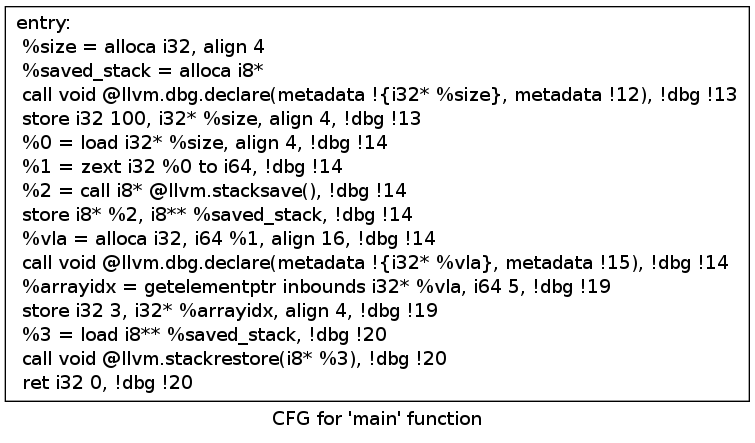
\includegraphics[scale=.25]{simple-before.png}
\caption{A basic block before bounds checking is added.}
\end{figure}

\begin{figure}
\label{fig:afterBounds}
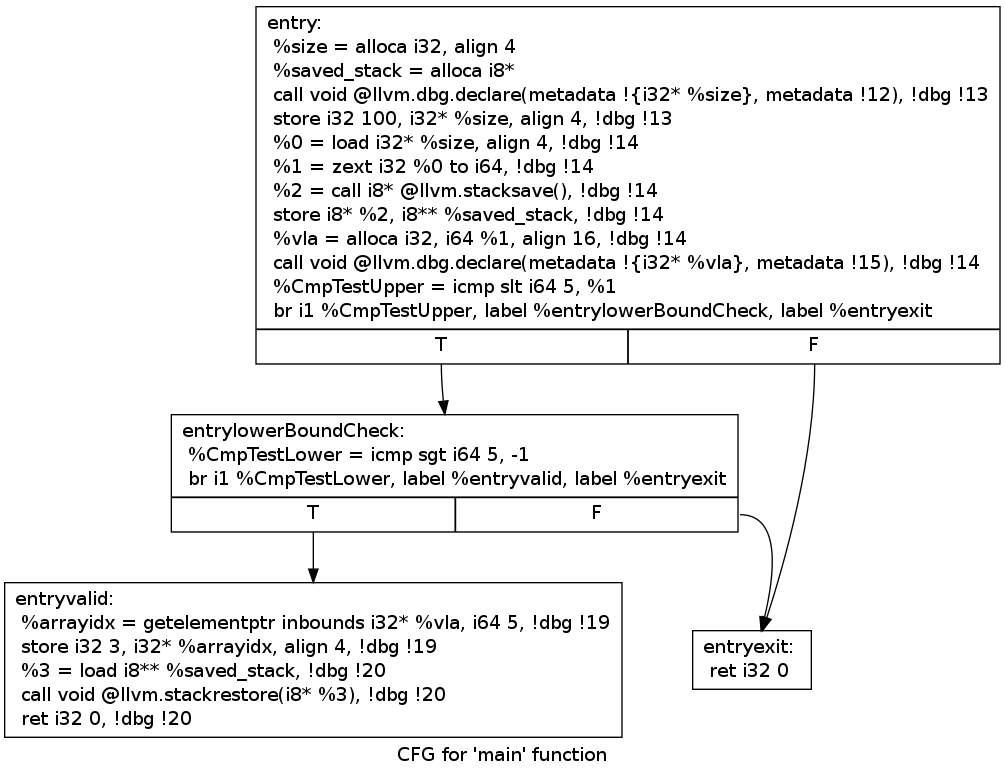
\includegraphics[scale=.25]{simple.png}
\caption{A group basic blocks after bounds checking is added.}
\end{figure}

\subsection{Optimized}

Once baseline is working, we want to optimize the run time checks. Those checks require additional instructions in the code, which will increase the program size and running time. Thus we want to keep these checks to a minimum. Our goal for this part of the project is to find and remove redundant bound checks.

Firstly, busy checks, checks where a comparison is anticipatable on all successors of the block it locates, are identified through backwards data flow analysis. Bound checks are copied to these locations to facilitate the removal of redundant checks on divergent branches.

Then we find the availability of the bound checks using a forward data analysis. A compare statement is killed when one of the variables in the compare statement are changed. A definition is available in a block if it is also available in all predecessors of that block. The output definitions of a block equals the set of all the input definitions excludes the definitions that have been killed and then intersects the set of generated definitions.

To optimize the reaching definitions of the compare statements even further, we have made some small adjustments. If an index has increased after the last check on that index, we kill the upper bound check, which means replacing it with a new one, but keep the old lower bound check. Likewise, if the index variable is decreased, we keep the upper bound check but kill the lower bound check. 

The next aspect of this optimization was removing redundant bounds checks. The algorithm iterates through each instruction in a block looking for generated compares that are identical to comparisons in the available set. Comparison equivalence is determined by a combination of their predicate and operands. Operands are considered equivalent if their temporary variables were created by loading the same variable, and no other operations have been performed on them. 
In addition, we must ensure that the value loaded was not previously modified in the memory. We determine this by tracking the store instructions in each block. It is possible to examine the instruction that is being stored and find if it is an increase, decrease, or unknown value compared to the previous stored value. Based on these results, the bound check can be killed in the outgoing set.

\subsection{CFG Restructuring}
Once the previous optimizations were made, we want to make a few more optimizations. This is a two-step process. Firstly we restructured the CFG of the program. Then we used global value numbering to optimize the program including bounds. Doing the CFG restructuring prior to the global value numbering allows for more optimizations. 

So the first part is to restructure the CFG. Our goal of the restructuring is to minimize the number of places where there are multiple definitions of a variable reaching. This helps since it allows for more compile time optimizations, as locations that have multiple reaching definitions are more difficult to optimize. So we attempt to do restructuring as explained by Thakur and Govindarajan\cite{Thakur}. 

The first thing we do is to find the distance between any two blocks in the function. We implement this by using Warshall�s algorithm. The primary purpose of this is to figure out which block was reachable from whom. This is important in later parts of the restructuring. 

The next thing we do is to find all the reaching definitions at each point in the program.  This is done by using a typical iterative reaching definition analysis. We go through each block and find the reaching definitions at each point. At the end of the block we follow all the paths and copy the current reaching definitions to those blocks. If it is a backwards edge, we restart analysis from that point. 

While doing the reaching definition analysis, we also perform the killed definition analysis. A variable has its definitions killed when at a point in the program, different definitions for that variable come through different paths. In doing the reaching definition analysis, if we see a definition is being killed, we save it in a map structure that mapped the basic block with the variables killed. 

The next thing we searched for is when a variable is used within a block that has multiple reaching definitions for that variable. If we find such a variable, we map this basic block to the used variable.

The next step in restructuring is finding which blocks influenced whom.  We do this by going through the lists of all the killed variables and used variables. If we find an intersection between the killed variables of one block and the used variables of another block, we say that the one kills it influences the one uses it. With this, we find the region of influence. To find the region of influence, we use the information about who can reach what. The region of influence is all the blocks that the influencer node can reach and can reach the influenced node. 

The next step is the actual cloning. Since we have the list of the regions of influence, we duplicate them. We make replicas of those blocks for each predecessor the influencer node of the region of influence had. Once we made the clones, we have to do some modifications to the name of the temporary variables used within the blocks to prevent definitions being used that don�t exist on a path.  Then we have to fix up the pointers for the cloned region of influence. After the cloning, the terminators for each block still point to the original next block, rather than the one within the region of influence. This has to be fixed. In addition, pointers have to be fixed so that the CFG edges actually point to these clones. So the predecessors of the influencer node are made to each point to a clone. This completes the restructuring. 

So the next thing is global value numbering. We look for load instructions and binary instructions. When we get these, we add them to a vector. If a constant value is being used, it is added to the valueID table and given an ID which is stored in the vector. If it is a variable, we use its ID number from the valueID table. And when we get to a store, we perform certain actions to insert the expression into the global value number. Firstly we check if the hash table currently has the expression. The check is performed in a manner in which the order of the operands does not matter. If the expression is found, we look for the id it was given. Then we give the variable the ID which that expression is assigned to. Otherwise we give this expression a new ID and store it in the hash table. We try to replicate the SSA form as much as possible. Each store instruction has its own id. In addition, we maintain a phi table that is constructed with the help of reach definitions. 

The last part of this is using this information to optimize the program.  One is for general store instructions.  If we are storing the outcome of an expression to a variable, and we find in the hash table that the expression has already been evaluated, we simply replace all the instructions relating with the evaluation of the expression with a load of the variable that has the result of the expression and store it in the variable waiting for the evaluation.  
The other aspect of the optimization is related with bound checks. We are trying to consider the times when we have a bound check reaching. It is for a different, but equivalent variable. We replace the bounds check with a new one, in which we find the first combination of those operands equivalent. Thus all equivalent bound checks will look the same. Afterwards, when we run the pass developed in part 2, the redundant ones will be deleted. 

\section{Limitations}
\subsection{Baseline}
The major limitation of our approach with baseline is that dynamic allocations cannot be examined. If an array was created via a malloc, we cannot detect or analyze it. Also, it only works with 1D arrays.

\subsection{Optimized}
The most serious limitation of this part of the project is that we cannot always tell if we should kill an bounds check. Similar to normal reaching definitions, we have to take the safe approach and kill a definition if we are unsure of whether or not it reaches. For example, if we add a runtime value to our variable, both bounds checks will have to be killed as it is not possible to determine the sign of that runtime value.

Additionally, the version of LLVM currently being used has a limited ability to recalculate the dominator tree during other transformations. Due to the restructuring that was added because of the additional compares and branches, we were not able to recalculate the dominator tree. This means we are only able to copy �busy checks� to blocks previously known to the dominator tree analysis.

\subsection{CFG Restructuring}
We have quite a few limitations with the implementation of this optimization.  The first one is that it does not work with loops. The major limitation is that if there is an area that needs to be cloned within another area that needs to be cloned, the CFG restructuring may malfunction. It will not make enough clones since one clone is not aware of the other. Thus this is a major limitation. Another limitation is that after a region is cloned, any definitions created there are treated as duplicates, even if they are in fact not. So if a definition $d = 5$ is created in both branches by a clone, on its use afterwards, the algorithm will detect multiple definitions for d and thus try to make another clone of d, which should not exist.  For this reason, such algorithm does not work with arrays, either.

Another limitation is that the global value numbering that we were using to do further optimizations in the bound checking as well as normal code is limited in its range. We were largely able to implement it, but there are a few small limitations. The primary one relates with phi instructions. We had to implement phi instructions ourselves, and thus we could not fully reach its potential. The primary thing is it can�t do phi equality between different variables. Another limitation is that after a clone, an expression that is generated and used within the cloned region is not available. A last limitation is that it does not work with arrays.

Currently this does not work in combination with the bound checking of part 1 and 2, due to the fact that those parts often cause temporary variable creation to be put in a different block than their use. When the restructuring was designed, this condition was not considered. This caused us unable to work with part 1 and 2. 

\section{Results}
\begin{table*}[t]
\label{tbl:results}
\begin{tabular}{|c|c|c|c|}
\hline
Implementation & Compile Time (s) & Run Time (s) & Code Size (kB)\\\hline
Original & N/A & 0.002466 & 4.2\\\hline
Baseline & 0.01514 & 0.00312 & 5.5\\\hline
Optimized & 0.0234 & .003 & 4.4\\\hline
CFG Restructuring & 0.06586 & 0.00344 & 7.1\\\hline
CFGRestructuring with Optimization & 0.11984 & 0.00357 & 10.25\\\hline
\end{tabular}
\caption{The benchmark results of each implementation.}
\end{table*}


\subsection{Baseline}

Adding in the bound checks for runtime and doing some compile time checking of bounds increased the compile time, run time and code size. Compile time increased because our Pass analyses the code and adds bound checking to the original code during compile time. These checking instructions also cause the code size to increase proportional to the percentage of array references in the original code. For our benchmark, it is roughly 23.8\%. Since these checkings are not memory accessing instruction (which is more time consuming and may cause stall) and the branching statement will not be taken unless the program fails the bound check and terminates, the run time does not increase as much as the code size does.

As mentioned, there are some compile time checks added. If both the bound and the index of the array are constants, we can do the check at compile time rather than add to the code by adding run time checks. You can see this occurring in the benchmark code in the entry block when we are indexing element 20 of 100 of array a on line 28. As you can see, we did not add any code within the program to handle this. This is simply handled at compile time since everything about this indexing is known then, and thus increases the compile time. This is actually already done in llvm, but we are doing it in our pass also. 

We also added several run time checks. Anytime we seen an array being indexed into, we add checks to the lower and upper bound. You can see this throughout our code in the form of  icmp instructions. This obviously leads to increased code size, and takes time to compile. There are 2 compare instructions and 2 branches added for each indexing. However, unless the code is very array heavy, as in almost every access is an array, it will not significantly alter the run time.  As you can see, if any of those tests for bound checking fail, they go to an exit block. Since we did not know how to throw an error, instead we branch to this block and cause the function to return. Otherwise they continue on the normal program flow. 

\subsection{Optimized}

Our optimization removes redundant bound checks in condition that the result of a bound check can be determined from available expressions and previous bound checks in compile time.\cite{GuptaFLO} The elimination of redundant checking statements reduces the code size and run time. Compared to the output of the baseline bound check, about 85\% bound checking statements are eliminated for our benchmark code.

As can be seen in the CFG for the benchmark, there were optimizations made in the bound checks. In the benchmark, there is a section where we have two instructions indexing into $b$, $b[y] = c2$, and $b[y] = c1$. Looking at the CFG for this test, from ifend to ifendvalidvalid, it can be seen that the bound checking for y the second time are optimized out.

To maximally show the benefits of this code, we ran a second test. This is labeled as benchmark2.cpp in test folder. In this, there are two arrays $i$ and $j$. $i$ is initially indexed with $x$. Thus both lower and upper bound checks were done. $i$ then decreased in value. The optimization that part 2 made was that the upper bound check was removed because $i$ had decreased.  However, the upper bound check was kept. For $j$, we did the opposite. We indexed with $y$, and the initial array access, there were tests for both lower and upper bound. However, $y$ then was increased, thus the lower bound check was removed. 

\subsection{CFG Restructuring}

According to our test result, including the CFG Restructuring algorithm causes a significantly longer compile time.  The code size grows about 69\% from the original and the runtime increases accordingly. Such behavior fits what we expected. Compile time is increased because there is a significant amount of processing needed in compile time to support the restructuring and global value numbering. To support them, there is an increase in code size, leading to a larger file. In addition, there are some instructions added to help in the restructuring, which lead to the slightly higher run time. 

As can be seen by the resulting CFG, there is a significant amount of duplication that is done. Areas between where multiple definitions of variables are created and where there are used are duplicated.  This helps significantly when doing global value numbering. For example, after the first if then statement, we are able to use global value numbering to optimize the evaluation of the expression c5-c1 in line 38 of the benchmark. This is only evaluated in one part of the if-then statement, and is reused after. The restructuring generates  a clone for both the then and else part of the if-then. Because of this, in the clone following the if-then where this evaluation is first calculated, we can reuse that calculation rather than recalculating. As can be seen, we were not able to make this optimization in the if-else part of the clone because that block did not evaluate the expression.

 You can see further examples of how global value numbering is useful. These cases are not helped by the restructuring though. $z + 5$ is evaluated in the first block, line 25 of the benchmark. It is then again used in the block following the first if-then statement, in lines 41 and 43. It can be seen that the first evaluation is used to put the value into r. You can also see that once z was redefined, we no longer could use it. 

Another place you can see the importance of global value numbering and how it helps when restructuring is with the compare statements in the if-then statements. With global value numbering, whenever we see an if-then statement, we modify the icmp instruction associated with it. We look up the values being used and take the first equivalent variable to each value. As we mentioned before, this ensures that all equivalent icmps will thus use the same value and bound. This makes it easier to optimize a latter icmp out. For example the last two if statements, $y>5$ and $x>5$ are equivalent, as it is stated that $y=x$. Thus you can see that in block ifend28clone1 has the same compare statement as that in ifend. You can see the same behavior in its clone of those blocks created in restructuring. ifendclone, ifend28clone, and ifend28cloneclone all do a comparison between c2 and c5, even though they are a mix of comparisons of $y>5$ and $x>5$.  You will also see that ifend28 and ifend are not the same as $y$ used to be equal to i, but in that area of the restructuring, i changed values in ifthen12, because before we had changed $y>5$ to be a comparison between i and 5, but now that i changed values, this comparison is no longer valid. So there are a few cases where even though expressions are equivalent, global value numbering will not modify the compare statements to be equivalent. 

This previously mentioned feature is what we were hoping to take advantage of when trying to optimize array bound checks. Similar to if statements, they use compare statements, so the concept is the same. The hope was that we would first run the part 1 code to insert bound checks, then run this code, and then run the part 2 code, to remove the redundant bound checks we created by making equivalent bound checks appear the same. However, it turned out that the code we wrote for this part does not work with the way the bound checks are inserted. However, we have tested it out and found that if we run part 2 after this part, the redundant checks that are created by equivalent comparisons in if statements are optimized out. 

\subsection{CFG Restructuring with Optimization}

This test was running the optimization pass after doing the restructuring. As can be seen, there were increases in all the parameters from the base. Since this is a combination of the other passes, the reasons for increases in all these parameters is for the same reasons as the other tests. 

As mentioned in the previous section, we were unable to optimize bound checks. However, by running the optimization pass after CFG restructuring, we were able to optimize out compare statements used by if statements.  This can be seen in the examples mentioned in the previous section.  To point out a specific example, if you take a look at ifend28clonevalidvalidvalid, there is no compare statement. This is because it has been optimized out because it has already been tested at \textbf{ifendclonevalidvalidvalid}.

\section{Conclusion}

In this paper we  have examined the implementation and effects of bound checking optimization. These bound checks provide additional aids for developers at the expense of compile time, run time, and executable size. Several implementations, such as those in \cite{Gupta:1993:OAB:176454.176507}\cite{GuptaFLO}
\cite{Thakur}, discuss how to minimize these penalties and allow the best mix of functionality and performance. Following those previous works, we have implemented bound check optimizations with redundancy removal and CFG restructuring. To analyze the improvement and expense of these algorithms, we ran the two checks separately and combined on a testing benchmark code, and compared the compile time, run time and output file size. The original code and the baseline bound checking without any optimization were included as control group. Our test result shows that compared to the baseline bound checking, the optimization significantly reduced the code size and run time at the expense of compile time.

\bibliography{bibliography}
\bibliographystyle{plainnat}

\end{document}
